\documentclass{article}

\usepackage{notes}
\usepackage{array}
\usepackage{amsmath}
\usepackage{mathtools}
\usepackage{graphicx}
\usepackage{amssymb}
\usepackage{enumitem}
\usepackage{textcomp}
\usepackage[hidelinks]{hyperref}
\usepackage[a4paper,margin=0.5in]{geometry}
\renewcommand\vec{\mathbf}

\graphicspath{{./Images/}}

\everymath{\displaystyle}
\DeclarePairedDelimiter{\ceil}{\lceil}{\rceil}

\begin{document}

\title{IVR Condensed Summary Notes For Quick In-Exam Strategic Fact Deployment }
\author{Maksymilian Mozolewski}
\maketitle
\tableofcontents

\pagebreak

\nChapter{Vision}

\nSection{Introduction to Vision}

\nDefinition{Computer vision}{Processing data from any modality which uses the electromagnetic spectrum and produces an image}
\nDefinition{Image}{Way of representing data in a picture-like format, with a direct correspondence to the scene being imaged}
\nDefinition{CCD Camera}{
    Charged couple device, light falls on an array of MOS capacitors (which are rectangular and not square). The capacitors form a shift register and output either a line at a time or the whole array at one time (line vs frame transfer)
    
    \centering
    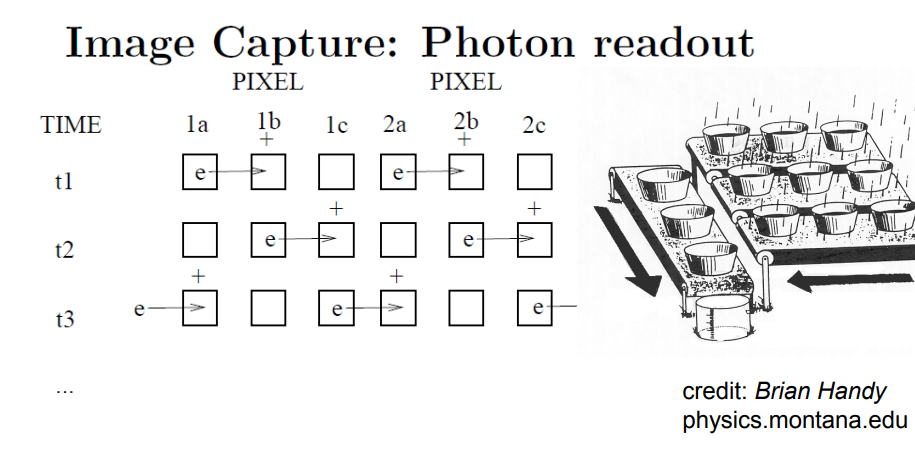
\includegraphics[width=0.5\columnwidth]{ccd_camera.png}

    \raggedright
    these "buckets" can overflow, resulting in over-saturation of the image
    }
\nDefinition{Frame grabber}{Device which converts analog image signals to digital image signals. Essentially puts a discrete value on each pixel signal. 24bit color is usually required for robotics}
\nDefinition{Visual Erosion}{RGB is a function of the sensitivity of the sensor to reflected light of each color. The sum of those intensities may vary wildly from frame to frame depending on the distance of the object due to intensity of the reflected light. The object appears to "errode" with changes in lighting. CCD Cameras are also notoriously insensitive to red, meaning that one of the three color planes is not as helpful in distinguishing colors. HSI and SCT colour spaces aim to reduce visual erosion since the Hue - the main wavelength measured (\textbf{perceptually meaningful dimensions}) will not change with the object's relative position, only its saturation and intensity will! Equipment to capture HSI images is expensive, and conversions between colour spaces sometimes fail.}
\nDefinition{Region Segmentation}{Finding groups of pixels related to each other via color, within a certain threshold and identifying the centroids of those groups. Requires high contrast between the \textbf{foreground} (object of interest) and the \textbf{background} to work well.}

\nDefinition{Color histogramming}{
    a type of histogram (bar chart basically), the user specifies range of values for each bar, 
    (bucket) the size of the bar is the number of data points falling within the bar's "range". 
    These ranges could be set to capture different values of either the R,G,B color intensities.

    \centering
    \includegraphics[width=0.7\columnwidth]{"histogram.png"}

    \raggedright
    Such histograms can be \textbf{subtracted bucket-wise} from each other as a form of distance measure to compare image stimuli.
}

\nDefinition{Stereopsis}{The method of triangulating depth data from 2 POV's}
\nDefinition{Stereo camera pairs}{Usage of two cameras to extract range data by finding the same point on the images received from two (most likely parallel) cameras, and then finding the depth information using the geometry of the cameras. It can be hard to find the same point on two pictures ()\textbf{correspondence problem}), the method of picking a spot of interest is called an \textbf{interest operator}. Cameras can be mounted in parallel to produce \textbf{rectified images} (the distance between the two cameras is then known as the \textbf{disparity}). This can save computation time since the point of interest will appear in the same line of the image on both cameras (\textbf{epipolar lines})}

\nDefinition{Optic flow}{Information to do with: Shadow cues, texture, expected size of objects}
\nDefinition{Light stripping}{
    Method of projecting a pattern of light onto a surface of interest and observing the distortion to the pattern to visualise the surface and/or distance information. Does not work that well in natural conditions due to noise.
    
    \centering 
    \includegraphics[width=0.4\columnwidth]{"light_stripper.png"}
    
}

\nDefinition{Laser ranging}{like radar but using light (\textbf{lidar}), scanning components are expensive, a planar laser range finder is a cheaper alternative. Produces an intensity and range map.}
\nDefinition{Range segmentation}{Segmenting the image based on range data, can be used to determine the geometry of surfaces}

\nSection{Image Basics}


\nTheorem{Homogenous coordinates}{
    Homogenous (aka similar) coordinates are coordinates in space with one more dimension than in the corresponding cartesian space, in this space we can express linear translations as linear matrix transformations!
    Every point in the cartesian space becomes a line in the homogenous space!

    \centering
    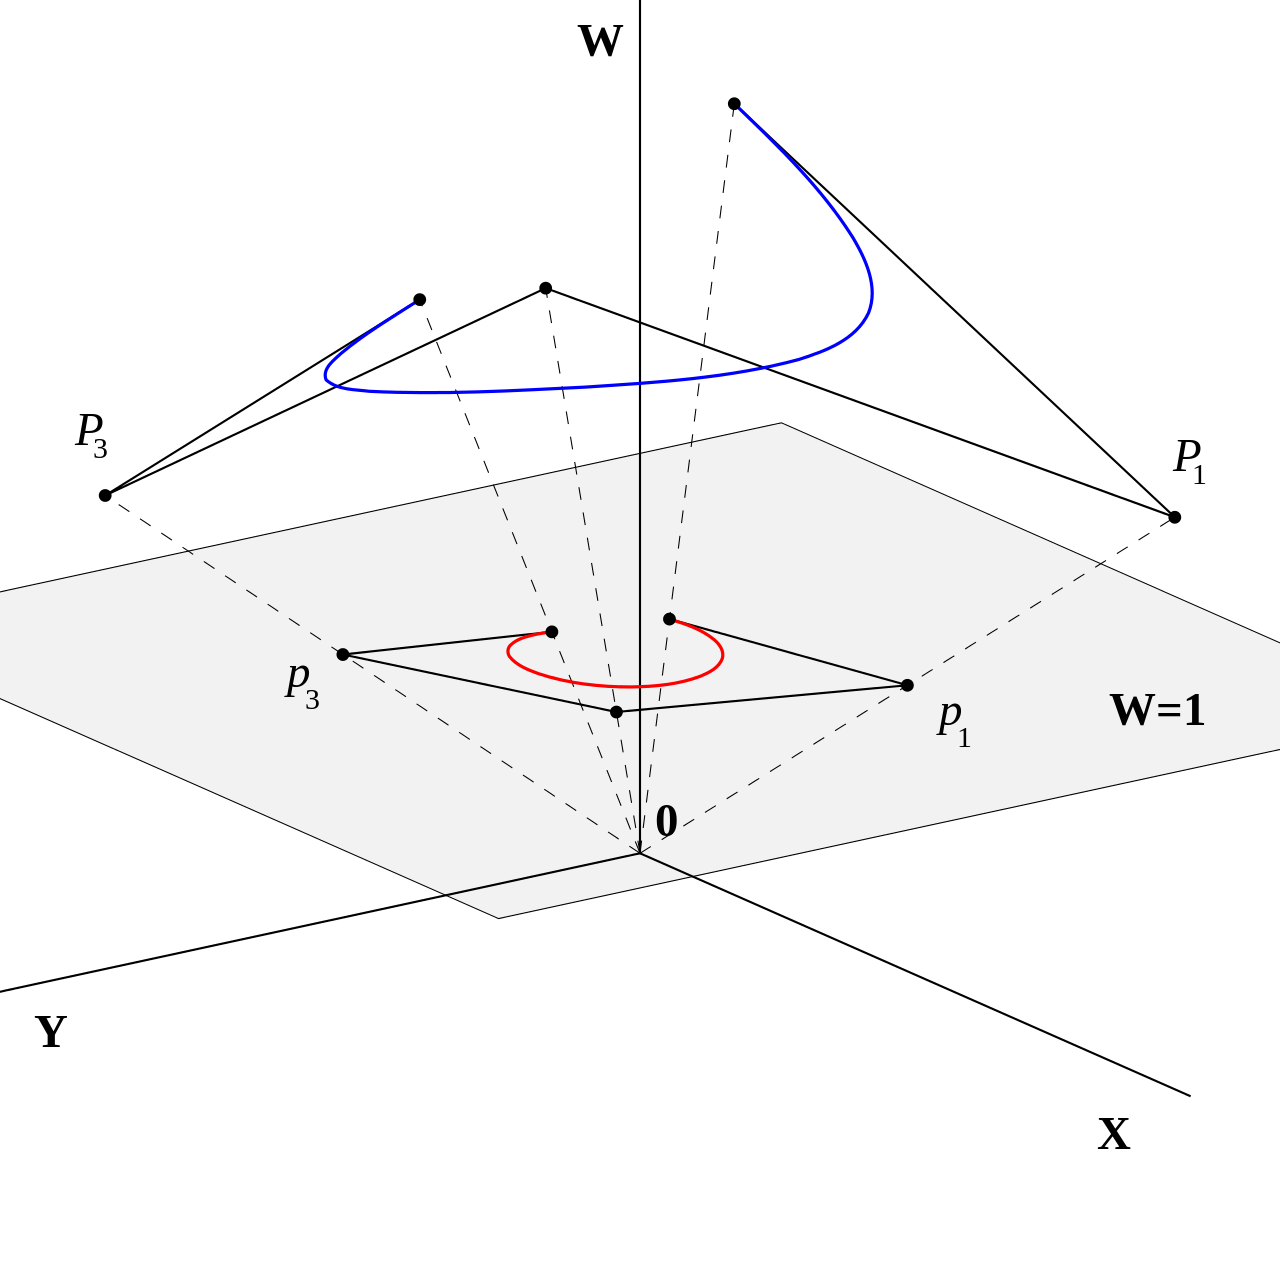
\includegraphics[width=0.5\columnwidth]{homogenous.png}

    \raggedright
    Conversion to homogenous coordinates:
    \begin{equation}
        \begin{bmatrix}
            x \\ y \\ \vdots \\  
        \end{bmatrix}
        = 
        \begin{bmatrix}
            x \\ y \\ \vdots \\ 1
        \end{bmatrix}
    \end{equation}

    Conversion from homogenous coordinates
    \begin{equation}
        \begin{bmatrix}
            x \\ y \\ \vdots \\ w
        \end{bmatrix}
        = 
        \begin{bmatrix}
            x/w \\ y/w \\ \vdots
        \end{bmatrix} 
        \quad w \neq 0
    \end{equation}

    Notice how a point in homogenous space can be multiplied by any constant, and yet when it is converted back to normal space, it becomes the same point. \textbf{The ratio} between the components defines the line in homogenous space.
}

\nTheorem{Pinhole camera}{
    
    Capturing on a simple plane does not work because multiple rays from the same point in the scene travel to multiple parts of the film. We want the film to capture a single "ray" per point of interest
    \begin{center}
    \begin{tabular*}{\columnwidth}{m{0.5\columnwidth}m{0.5\columnwidth}}
        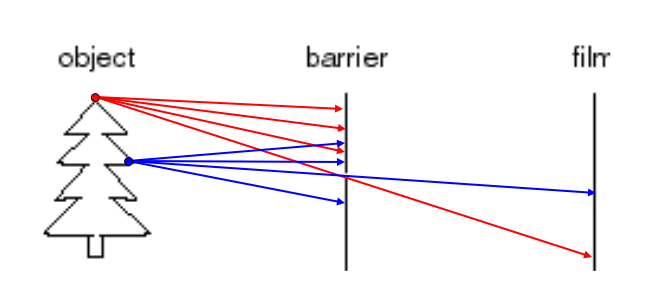
\includegraphics[width=0.45\columnwidth]{pinhole_failure.png}&
        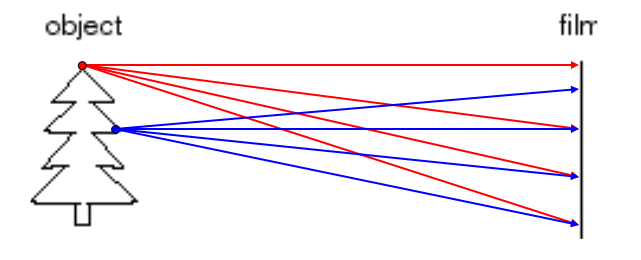
\includegraphics[width=0.45\columnwidth]{pinhole_failure_2.png}
    \end{tabular*}
    \end{center}

    A camera setup using a tiny hole to filter and hence focus the light onto a single clear image.

    \centering 
    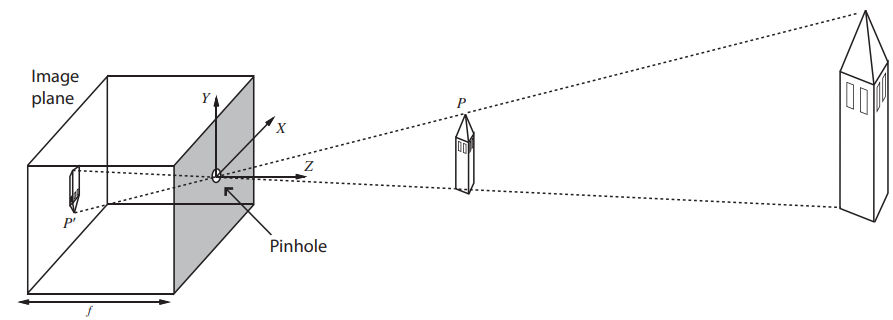
\includegraphics[width=0.6\columnwidth]{pinhole.png}
    
    \raggedright
    Using similar triangles, the point P:$(X,Y,Z)$ maps to point P' on the 2d surface of the image plane, at a distance f (\textbf{focal length}) from the pinhole as follows: 
    \begin{equation}
        x = \frac{-fX}{Z},
        y = \frac{-fY}{Z},
        z = f
    \end{equation}

    This projection of scene point to camera point can be expressed as a linear matrix transformation in homogenous space:

    \begin{equation}
        P_{h} =
        \begin{bmatrix}
            X \\ Y \\ -Z/f
        \end{bmatrix}
        =
        \begin{bmatrix}
            1 & 0 & 0 & 0 \\
            0 & 1 & 0 & 0 \\
            0 & 0 & -1/f & 0 
        \end{bmatrix}
        \begin{bmatrix}
            X \\ Y \\ Z \\ 1
        \end{bmatrix}
    \end{equation}

    To retrieve the projected point in cartesian space we simply divide by the third coordinate and discard it.

    \begin{equation}
        P_{c} = 
        \begin{bmatrix}
            X / (-Z/f) \\ Y / (-Z/f)
        \end{bmatrix}
        = 
        \begin{bmatrix}
            -fX/Z \\ -fY/Z
        \end{bmatrix}
    \end{equation}
    Which is identical to the projection above.

    This projection, preserves straight lines (\textbf{colinearity}) and their intersections, but looses information about angles and lengths (due to multiple points in 3D possibly mapping to the same point in 2D)
    
    Lines directly passing through the focal point are projected as points.
    
    Planes are preserved but those passing through the focal point are projected as lines.
}


\nTheorem{Vanishing point}{
    Any two parallel lines will converge to a certain point on the image as long as their directions are the same
    
    \begin{center}
    \begin{tabular*}{\columnwidth}{m{0.5\columnwidth}m{0.5\columnwidth}}
        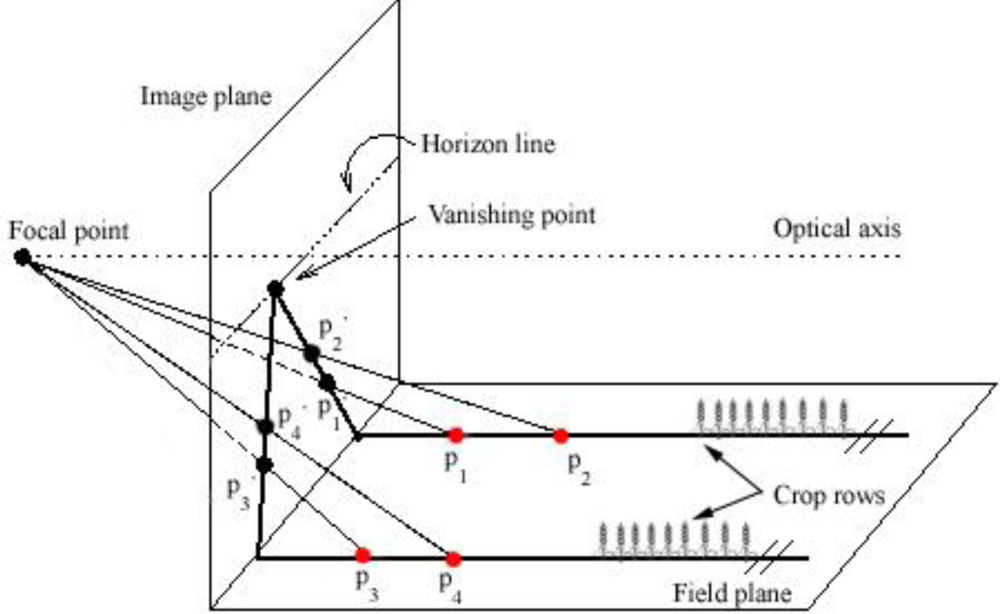
\includegraphics[width=0.45\columnwidth]{vanishing_point.png}&
        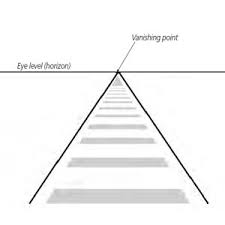
\includegraphics[width=0.45\columnwidth]{vanishing_road.jpeg}
    \end{tabular*}
    \end{center}
}

\nDefinition{Detector response curve}{
    The curve showing which frequencies of light a detector perceives the most and which will dominate the actual "perceived" or "central" wavelength of light, 
    i.e. the curve showing which wavelength of light a detector is most sensitive to.
    Each sensor type acts as a filter to the incomming light, and can produce an output signal proportional to the amount of its central wavelength absorbed.
    \\
    \par
    The wavelength signal perceived is a function of many things:
    \begin{itemize}
        \item type of source light
        \item the reflective properties of the objects in the scene 
        \item the sensor detector curve
    \end{itemize}

    As such knowing the "real" wavelength of the light is very difficult.
    
    \begin{center}
    \begin{tabular*}{\columnwidth}{m{0.5\columnwidth}m{0.5\columnwidth}}
        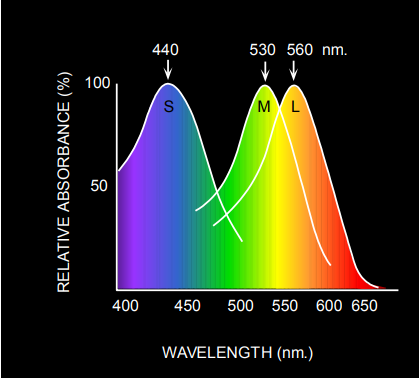
\includegraphics[width=0.45\columnwidth]{sensor_curves.png}&
        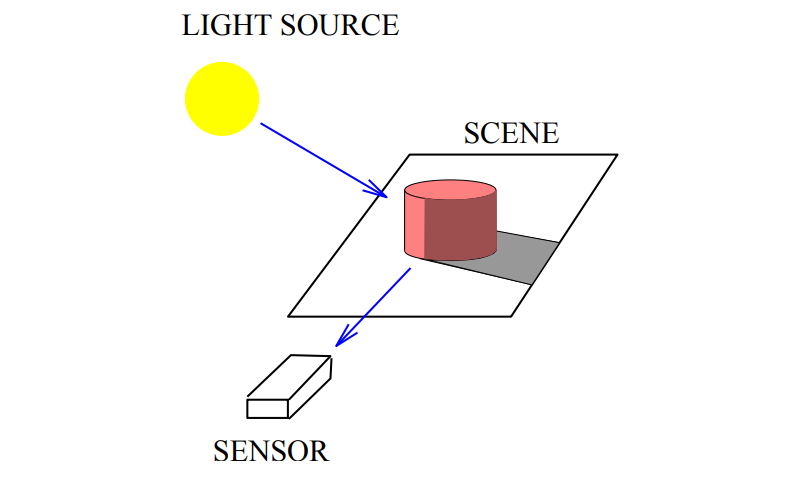
\includegraphics[width=0.45\columnwidth]{sensor_function.png}
    \end{tabular*}
    \end{center}
}

\nTheorem{Homography}{
    An invertible linear transformation $\mathbf{P}$ that maps points from one plane to another (think of it as a change of POV)

    \centering
    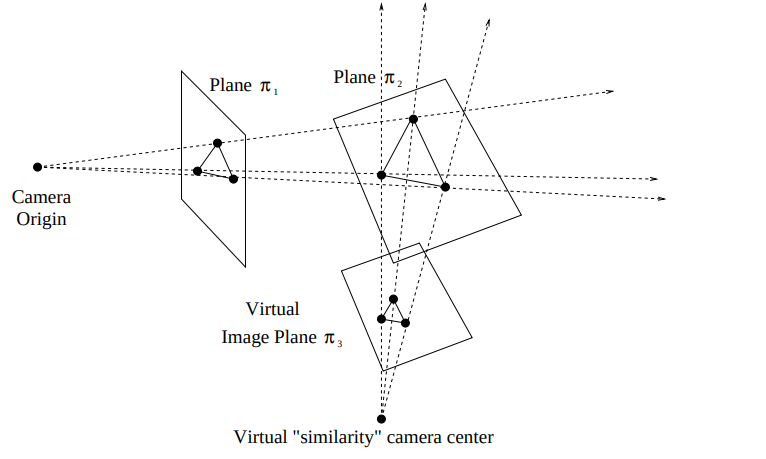
\includegraphics[width=0.8\columnwidth]{homography.png}

    \raggedright

    Given at least 4 corresponding points on each plane defining a POV, we can perform a least-square estimation of $\mathbf{P}$:
    \begin{equation}
        \mathbf{P} = 
        \begin{bmatrix}
            p_{11}&p_{12} &p_{13} \\
            p_{21}&p_{22} &p_{23} \\
            p_{31}&p_{32} &p_{33} 
        \end{bmatrix} 
    \end{equation}

    let $\vec{p} = (p_{11},p_{12} ,p_{13}
        p_{21},p_{22} ,p_{23},
        p_{31},p_{32} ,p_{33})$
        
    let $\mathbf{A}_{i} = 
        \begin{bmatrix}
            0 & 0 & 0 & -u_{i} & -v_{i} & -1 & y_{i}u_{i} & y_{i}v_{i} & y_{i} \\
            u_{i} & v_{i} & 1 & 0 & 0 & 0 & -x_{i}u_{i} & -x_{i}v_{i} & -x_{i} 
        \end{bmatrix}$
    
    construct $\mathbf{A} = 
        \begin{bmatrix}
            A_{1}\\A_{2}\\ \hdots \\ A_{N}
        \end{bmatrix}
    $

    Compute SVD($\mathbf{A}) = \mathbf{UDV'} $
    
    $\vec{p}$ is last column of $\mathbf{V}$ (eigenvector of smallest eigenvalue of $\mathbf{A}$)
    
    Then once we know the homography $\mathbf{P}$, then we can map (u,v) onto (x,y) using:
    \begin{equation}
        \begin{pmatrix}
            \lambda x \\ \lambda y \\ \lambda  
        \end{pmatrix}
        = \mathbf{P}
        \begin{pmatrix}
            u \\ v \\ 1
        \end{pmatrix}
    \end{equation}
    ($\lambda$ representing the fact that this coordinate is in homogenous space)

}

\nDefinition{Focus problems}{
    Focus set to one distance, and other nearby distances in focus (depth of focus). Further or closer not so well focused.
    
    \centering
    \nImg[0.6]{focus_problem.png}
    
    \raggedright
    Solutions: Use smaller aperture and brighter light
}

\nDefinition{Shadow problems}{
    False colours due to different intensity of light (shadows) make it difficult to separate shapes of interest from shadows.
    (is the white part under this part a shadow or the edge ?)

    Main cause of the problem: point of light sources, the perceived brightness at a surface is proportional to the \textbf{square} of the distance between the surface and the light source.

    \centering
    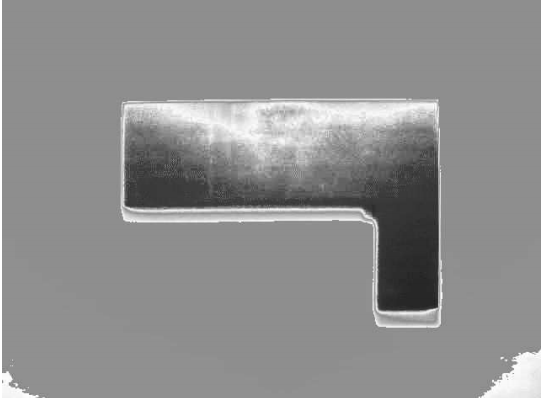
\includegraphics[width=0.3\columnwidth]{shadow_problems.png}
    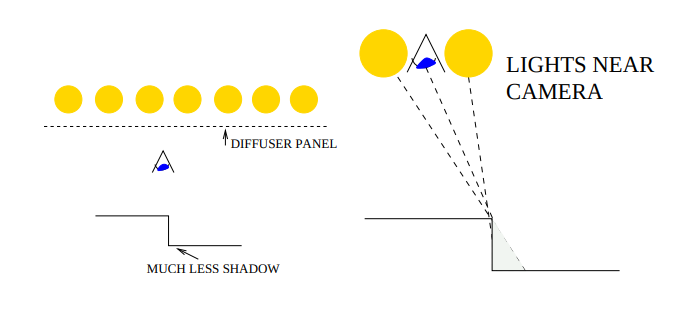
\includegraphics[width=0.6\columnwidth]{diffuser_panels.png}

    \raggedright
    Solutions: increase ambient lighting by using diffusing panels or lots of point lights
    }

\nDefinition{Specularities/highlights}{
    (Saturated pixels set to red)

    \centering
    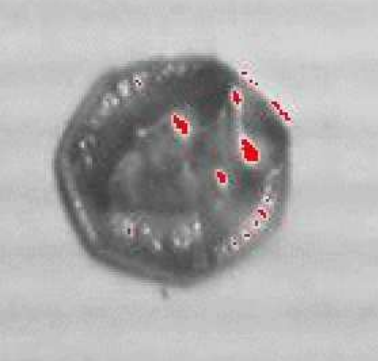
\includegraphics[width=0.3\columnwidth]{specularities.png}
    
    \raggedright
    Solutions: increase ambient lighting by using diffusing panels or lots of point lights, or use smaller aperture, reduce gain and adjust gamma
    
}

\nDefinition{Non-uniform ilumination}{
    Contrast on background enhanced: may cause analysis problems

    \centering
    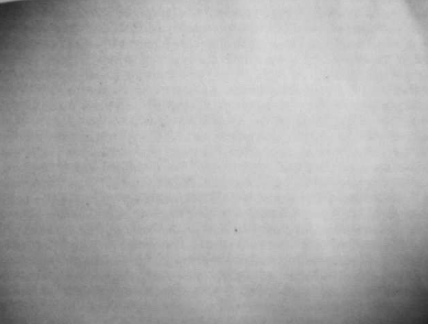
\includegraphics[width=0.3\columnwidth]{non-uniform-ilum.png}

    \raggedright
    Solutions: increase ambient lighting by using diffusing panels or lots of point lights
    
}
\nDefinition{Radial lens distortion}{

    Lenses sometimes slightly distort the image "radially" making accurate measurements hard
    \nImgs[0.35]{radial-lens-distor.png}{lens-distortion-graphic.jpg}

    Solutions: more expensive lenses, view from further away
}

\nSection{Image Segmentation}
\nDefinition{Approaches}{
    Image segmentation is the process of grouping pixels which belong together semantically, i.e. perhaps because they belong to the same object.

    We can segment based on many facts:
    \begin{itemize}
        \item Contrast - objects have different lightness : use thresholding
        \item Change - objects different from background : background models 
        \item Similarity - objects have consistent colours : colour clustering
    \end{itemize}
}

\nDefinition{Thresholding}{
    This method assumes that pixels are separable based on their color values. We can pick threshold boundaries for each color value and select regions based on 
    regions of pixels which fall in those boundaries.

    \centering
    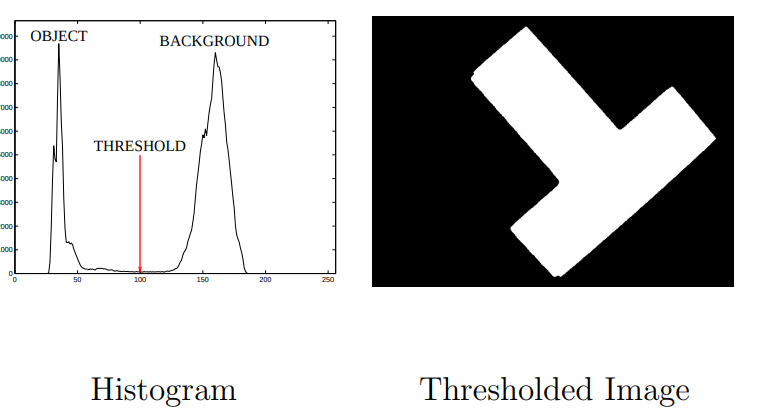
\includegraphics[width=0.8\columnwidth]{thresholding.png}
    \raggedright

    problems:
    \begin{itemize}
        \item Distributions may be broad and have some overlap leading to misclassified pixels
        \item variations in lighting might cause parts of the object to be missing, or shadows to be classified as objects
        \item color distributions might have more than 2 peaks
    \end{itemize}
}

\nDefinition{Convolutions}{
    General-purpose image (and signal) processing function.

    can be used to remove noise, smooth data, or detect features!

    In the case of thresholding, we can use convolutions to smooth the histogram.
    Imagine convolutions as a sliding window, where each point in the original image is replaced with the weighted average of the window at that position with the pixels.

    \centering
    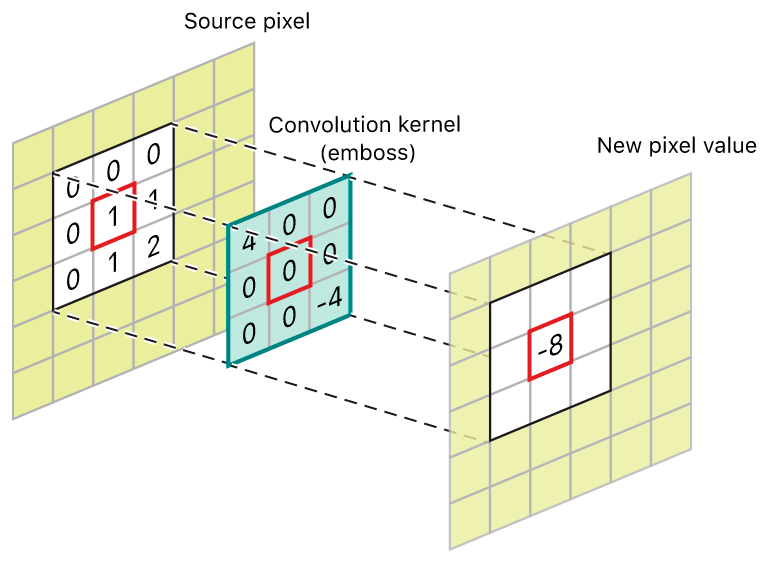
\includegraphics[width=0.8\columnwidth]{convolution.png}

    \raggedright

    Convolution in 1D, with kernel of size (odd) N (even kernels require padding with zeros):
    \begin{equation}
        \textit{Output}(x) = \sum_{i = -\lfloor N/2 \rfloor}^{\lfloor N/2 \rfloor} \textit{weight}(i) * \textit{input}(x - i) 
    \end{equation}

    \centering
    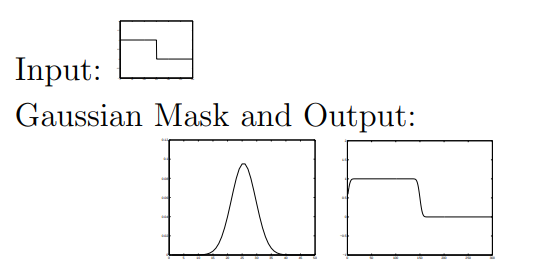
\includegraphics[width=0.5\columnwidth]{convolution_example.png}
    
    \raggedright
    Convolution in 2D, with kernel of size (odd) N:
    \begin{equation}
        \textit{Output}(x) = \sum_{i = -\lfloor N/2 \rfloor}^{\lfloor N/2 \rfloor}\sum_{j = -\lfloor N/2 \rfloor}^{\lfloor N/2 \rfloor} \textit{weight}(i,j) * \textit{input}(x - i,y-j) 
    \end{equation}
}

\nDefinition{Smoothing kernel (2d gaussian)}{
    \centering
    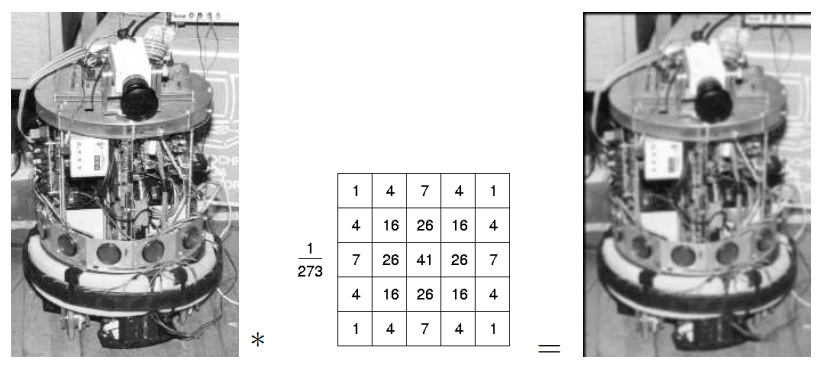
\includegraphics[width=0.9\columnwidth]{smoothing_kernel.png}
}

\nDefinition{Edge Detection kernel}{
    \centering
    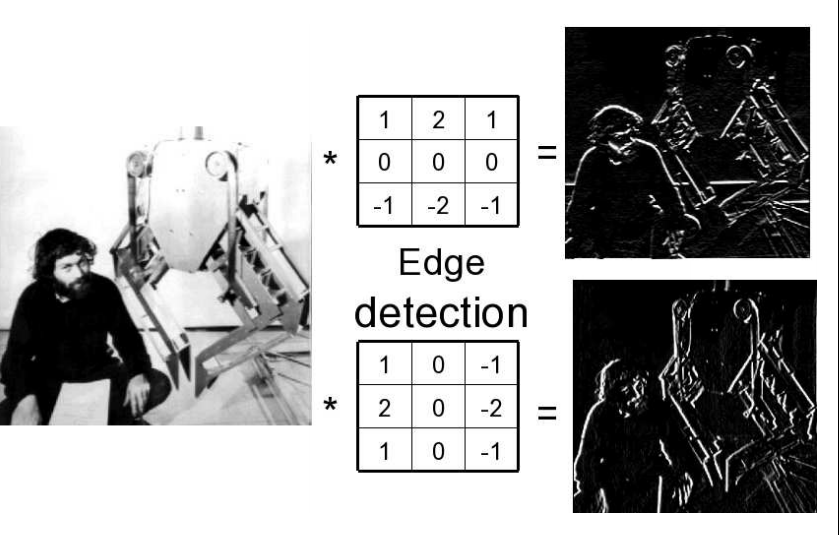
\includegraphics[width=0.9\columnwidth]{edge_detection_kernel.png}

}

\nDefinition{Background removal}{
    If we have 2 images, one with just the background (\textbf{B}) and one with background and foreground (the image \textbf{I}), we can

    \begin{equation}
        N = I - B       
    \end{equation}
    
    This difference will zero-out pixels with identical values to the background, and only leave those values which are different (either positive or negative depending on if the foreground is brighter or darker than the background at each point)

    We can do this for each channel of the image, and perform thresholding on the logical or between all the resulting differential pictures.

    \centering 
    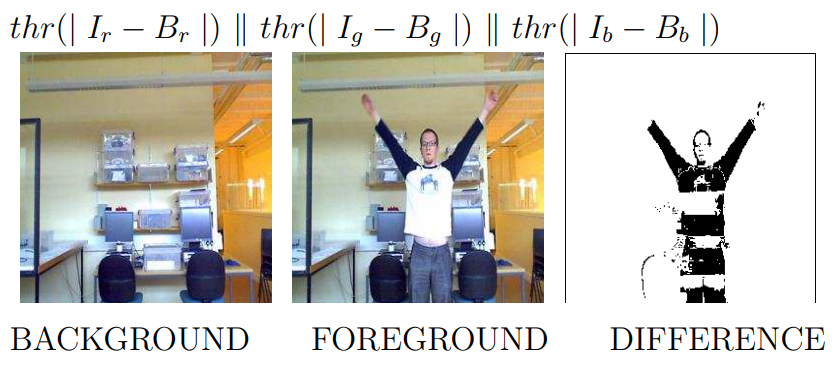
\includegraphics[width=0.7\columnwidth]{bg_differencing.png}

    \raggedright

    we can also use division instead of substraction to achieve a similar effect:
    \begin{equation}
        N = I / B
    \end{equation}

    This in effect removes the effects of illumination since:

    \begin{equation}
        \textit{background}(i,j) = \textit{illumination}(i,j) \cdot \textit{bg\_reflectance}(i,j)
    \end{equation}
    \begin{equation}
        \textit{object}(i,j) = \textit{illumination}(i,j) \cdot \textit{obj\_reflectance}(i,j)
    \end{equation}

    The pixels with a value of 1 are going to be the background, pixels with value $>$ 1 are lighter objects and pixels with values $<$ 1 are darker objects (than the background)

    In both of these techniques, we might need to use an operator such as the \textbf{open} operator to remove noise artifacts (with values which are just around the values which signify background pixels but not quite)

    Neither will work well when the background in I and B varies wildly.

}

\nDefinition{RGB Normalisation}{
    differences in lighting can be dealt with by normalising the RGB values of the image:

    \begin{equation}
        (r',g',b') = (\frac{r}{r+g+b},\frac{g}{r+g+b},\frac{b}{r+g+b})
    \end{equation}

    since multiplying all values r,g,b in the original space by a constant, changes the brightness of the color, we remove this effect thanks to the equation above,
    mapping all different brightness values of the same colour to one value.

    \centering
    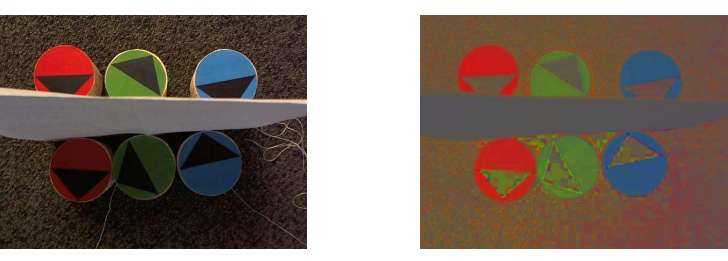
\includegraphics[width=0.5\columnwidth]{rgb_normalisation}
}

\nDefinition{Mean Shift Segmentation}{
    We can segment the image by performing clustering on the pixels by their color values (or any attributes for that reason)!

    The algorithm works as follows:

    \begin{enumerate}
        \item create a feature space over the attributes chosen to represent each pixel (for example for a grayscale this could be a 1d intensity axis)
            \newline 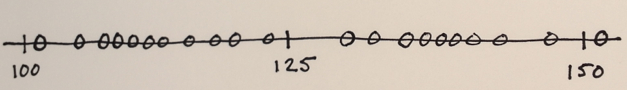
\includegraphics[width=0.7\columnwidth]{msc_0.png}
        \item distribute a number of "search windows" or kernels over the space 
            \newline 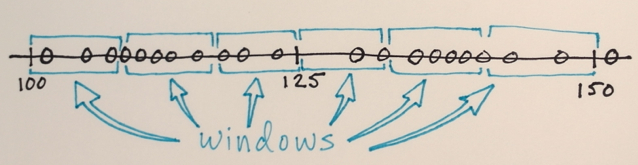
\includegraphics[width=0.7\columnwidth]{msc_1.png}
        \item calculate each window's mean 
        \item shift the center of each window to its mean 
            \newline 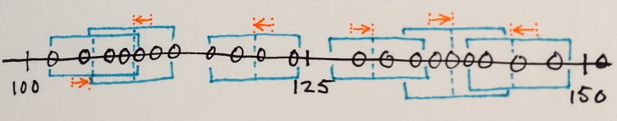
\includegraphics[width=0.7\columnwidth]{msc_3.png} 
        \item repeat steps 3-4 until convergence 
            \newline 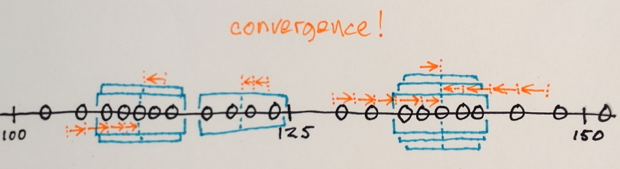
\includegraphics[width=0.7\columnwidth]{msc_4.png}
        \item merge windows ending up in close-enough locations, and call these the clusters
        \item cluster each pixel according to which cluster its original window ended up at 
            \newline 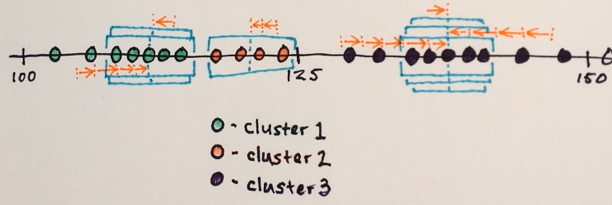
\includegraphics[width=0.7\columnwidth]{msc_5.png}
    \end{enumerate}

    the feature space can contain any number of dimensions, and so we could include spatial, color, texture-data, and so on. This is a very versatile algorithm.
    It is application-independent, model-free (does not assume any shape of clusters),
    only requires a single parameter (window size h) which affects the scale of the clustering
    It is robust to outliers and finds a variable number of modes given the same h.

    The output is heavily dependent on the window size h, however. And the selection of h is not trivial. The whole algorithm is rather expensive and does not scale well with the dimension of the feature space.
    }

\nSection{Description of Segments}

\nDefinition{Shape}{

    a set of points in the plane, or a continuous outline (silhouette)

    \centering
    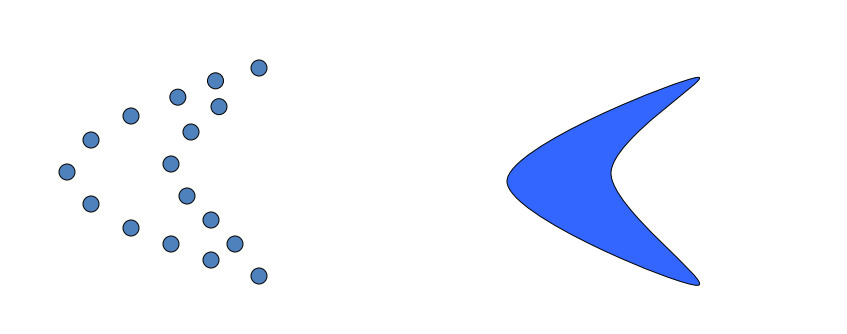
\includegraphics[width=0.5\columnwidth]{shape.png}

    \raggedright

    \nHeader{Cues}

    shapes can give us cues (\textbf{interior} and \textbf{boundary} cues)about the objects they outline.

    Some classes are defined purely by the boundary of the shape, some are defined purely by the \textbf{contents/interior} of the shape (i.e. texture,color), and some are defined by a mixture of both

    \nHeader{Correspondence and recognition}

    We can draw conclusions about similarities between shapes using \textbf{point-to-point} correspondences or \textbf{shape characteristics} to help us recognize objects belonging to certain classes.

    \centering
    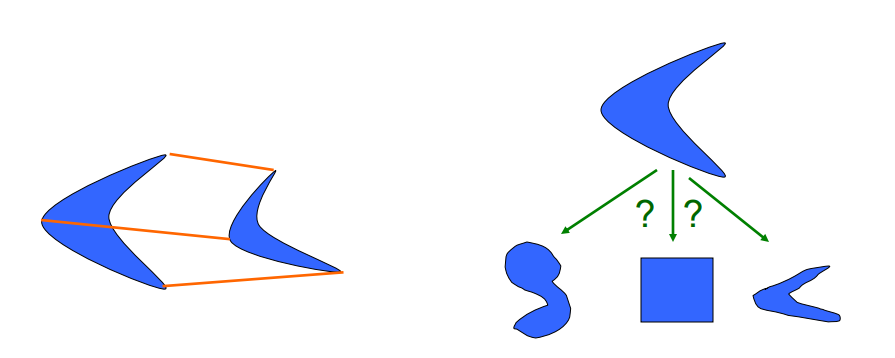
\includegraphics[width=0.7\columnwidth]{correspondence_recognition.png}

    \raggedright

    Good methods of finding similarities will be :
    \begin{itemize}
        \item Invariant to rigid transformations like: translation, rotation and scale
         \newline \nImg[0.4]{invariance_rigid.png}
        \item Tolerant to non-rigid deformations
         \newline \nImg[0.4]{tolerance_non-rigid.png}
    \end{itemize} 
    }


\nDefinition{Global shape descriptors}{
    Shape descriptors which put a number of a certain characteristic of a shape based on its \textbf{entirety} - hence "global".

    \nHeader{Convexity}

    Convexity describes the ratio of a shape's convex hull to its perimeter, values of 1 mean that the shape is entirely convex, and values $<$ 1 mean the shape is less convex.
        \begin{center}
        \nImg[0.2]{convexity.png}
    \end{center}
    \begin{equation}
        \textit{conv} = \frac{P_{\textit{hull}}}{P_{\textit{shape}}}
    \end{equation}

    \nHeader{Compactness}
    Compactness describes how close the perimeter of the shape is to the perimeter of the circle with the same area.
    \begin{itemize}
        \item If the circle of equal area has a smaller perimeter, this value will be smaller than 1, meaning that the shape's "mass" is distributed in a less compact manner.
        \item If the circle of equal area has equal parimeter, this value will be equal to 1, meaning the shape's "mass" is distributed as compactly as possible.
        \item This value cannot be greater than 1, as the circle is the most compact distribution of mass
    \end{itemize}
    \begin{center}   
        \nImg[0.2]{compactness.png}
    \end{center}
    \begin{equation}
        \textit{comp} = \frac{2\sqrt{A\pi}}{P_{\textit{shape}}}
    \end{equation}


    \nHeader{Elongation}

    The elongation is simply the ratio of the principal axes, i.e. the aspect ratio of a shape, this value can be anywhere between 0 (flat line) and $\infty$ (also flat line)
    This can be computed by taking the cross product of the principal axes with their length being set to the eigen values of the covariance matrix (if you treat each pixel as a data point)
    \begin{center}
        \nImg[0.2]{elongation.png}        
    \end{center}
    \begin{equation}
        \textit{elong} = \frac{c_{yy} + c_{xx} - \sqrt{(c_{yy}+c_{xx})^{2} -4(c_{xx}c_{yy} - c_{xy}^{2})}}
                                {c_{yy} + c_{xx} + \sqrt{(c_{yy}+c_{xx})^{2} -4(c_{xx}c_{yy} - c_{xy}^{2})}}
    \end{equation}

    \nHeader{Properties of these global descriptors}

    \begin{itemize}[noitemsep]
        \item[+] Invariant to translation/rotation/scale (rigid)
        \item[+] Robust to shape deformations (non-rigid)
        \item[+] Simple 
        \item[+] Fast to compute  
        \item[-] These do not find any point correspondences, 
        \item[-] Little power to discriminate between shapes (Can you discriminate between the shape of a horse and a plane with these ?) 
    \end{itemize}
}


\nDefinition{Moments}{
    Moments in mathematics are measures which put a number on the function of interest's graph. A shape can be thought of like the graph of some function defined on the 2D space (\textbf{f(x,y)}) 

    Family of stable \textbf{binary} (and grey level) shape descriptions which can be made invariant to translation, rotation and scaling

    Let $p_{yx}$ be the pixel value $ \in {0,1}$ at row y and column x

    Area $A = \sum_{y}\sum_{x}p_{yx}$
    
    Center of mass $(\hat{y},\hat{x}) = (\frac{1}{A}\sum_{y}\sum_{x}y \cdot p_{yx},\frac{1}{A}\sum_{y}\sum_{x}x \cdot p_{yx})$ i.e. average of x and y values weighted by "mass"

    \nHeader{Translation invariant}

    let $u,v \in \mathbb{Z}$

    then a family of 'central' (translation invariant) moments can be defined as:
    \begin{equation}
        m_{uv} = \sum_{y}\sum_{x}(y - \hat{y})^{u}(x - \hat{x})^{v}p_{yx}
    \end{equation}

    notice how with $u,v = 2$ this is somewhat similar to variance and a little close to the moment of inertia ($\sum_{p} mr^{2}$). This moment encapsulates the distribution of points around the center of mass, thanks to this 
    it does not matter where the shape is positioned.

    \nHeader{Scale invariant}

    We can make this family of moments invariant by noticing the fact that if we double the dimensions uniformly, then the moment $m_{uv}$
    increases by a factor of $2^{u}2^{v}$ w.r.t weightings ($y - \hat{y},x - \hat{x}$) and its area increases by 4.
    Hence $A^{\frac{u+v}{2}+1}$ grows by a factor of $4 \cdot 2^{u}2^{v}$,
    Therefore the ratio:
    \begin{equation}
        \mu_{uv} = \frac{m_{uv}}{A^{\frac{u+v}{2}+1}} = \frac{m_{uv}}{m_{00}^{\frac{u+v}{2}+1}}
    \end{equation}
    is invariant to scale (it cancels out the effects of increasing area, i.e. area = 1)

    \nHeader{Rotation invariant}

    We can generate a similar moment using complex numbers and multiple scale-invariant moments which is invariant to rotation:

    let $c_{uv} = \sum_{y}\sum_{x}((y - \hat{y}) + i(x - \hat{x}))^{u} ((y - \hat{y}) - i(x - \hat{x}))^{v}p_{yx}$
    
    then let:
    \begin{equation}
        \begin{aligned}
            &s_{11} = c_{11}/A^{2} \\
            &s_{20} = c_{20}/A^{2} \\
            &s_{21} = c_{21}/A^{2.5} \\
            &s_{12} = c_{12}/A^{2.5} \\
            &s_{30} = c_{30}/A^{2.5} \\
        \end{aligned}
    \end{equation}

    we can combine these to get rotation invariant descriptors in similar magnitudes like so:
    \begin{equation}
        \begin{aligned}
            &ci_{1} = \textit{real}(s_{11}) \\
            &ci_{2} = \textit{real}(10^{3}\cdot s_{21} \cdot s_{12}) \\
            &ci_{3} = 10^{4} \cdot \textit{real}(s_{20} \cdot s_{12}^{2})\\
            &ci_{4} = 10^{4} \cdot \textit{imag}(s_{20} \cdot s_{12}^{2})\\
            &ci_{5} = 10^{6} \cdot \textit{real}(s_{30} \cdot s_{12}^{3})\\
            &ci_{6} = 10^{6} \cdot \textit{imag}(s_{30} \cdot s_{12}^{3})\\
        \end{aligned}
    \end{equation}

    }

\nDefinition{Shape signatures}{
    We can represent the shape using a 1D function (\textbf{f(t)}) defined via the points on the boundary of the shape.
    Once we have such descriptors, we can establish similarity between two shapes using: $\int f(t) - f(t')$ i.e. the difference between the shape's descriptors integrated over t
    \nHeader{Centroid distance}

    for angle $t$, and point on boundary at that angle $p(t)$
    \begin{equation}
        \textit{r}(t) = d(p(t),\textit{centroid}) 
    \end{equation}
    \begin{center}
        \nImg{centroid_distance}    
    \end{center}

    \nHeader{Curvature}
    for angle $t$, and angle $\theta$ representing the angle between points $p(t)$ and $p({t+\Delta t})$ on the boundary at the angles $t$ and $t+ \Delta t$
    \begin{equation}
        k(t) = d\theta/dt
    \end{equation}

    \begin{center}
        \nImg{curvature_descriptor}
    \end{center}

    \nHeader{Properties of shape signatures}

    \begin{itemize}[noitemsep]
        \item[+] invariant to translation,scale(if shape is normalized), rotation (if orientation is normalized)
        \item[+] point correspondences (if both descriptors are aligned)
        \item[+] informative 
        \item[+] deformations affect signature locally  and not globally (i.e. at a single point of the signature)  
        \item[\texttildelow] manages to handle shape deformation to some degree
        \item[-] where to start t ? high computational cost of alignment of two signature functions
        \item[-] sensitive to noise (especially with derivatives)  
    \end{itemize}
}


\nDefinition{Shape Context}{
    Shape context is a shape descriptor utilizing the local properties of points on the boundary of each shape to establish \textbf{point-to-point} correspondences

    We do this by counting the number of other points around the points on the boundary of each shape in each bin of a polar-coordinate "kernel" (this forms a histogram)
    \begin{center}
        \nImgs{shape_context_descriptor_polar.png}{shape_context_descriptor}
    \end{center}

    We can compare the K-bin histograms $h_{i}(k),h_{j}(k)$ of two points $i,j$ on different shapes respectively, using the chi-squared test: 
    \begin{equation}
        C(i,j) = \frac{1}{2} \sum_{k=1}^{K}\frac{(h_{i}(k) - h_{j}(k))^{2}}{h_{i}(k) + h_{j}(k)}
    \end{equation} 
    This establishes a cost function over which we can pair-up the corresponding points on each shape, by finding the least-cost matching $\pi(p)$ of points on one shape to the other (perhaps using the hungarian or blossom algorithms)
    which minimizes the total cost:
    \begin{equation}
        H(\pi) = \sum_{p \in \textit{all\_points}} C(p,\pi(p))
    \end{equation}

    thus establishing a point-to-point correspondence between two shapes:
    \begin{center}
        \nImg[0.2]{point_correspondance}
    \end{center}

    \nHeader{Propertis of shape signatures}

    \begin{itemize}[noitemsep]
        \item[+] invariant to translation
        \item[+] invariant to scaling (if we normalize the radial distances between points in each shape by their mean)
        \item[+] informative - describes points in the context of the overall shape
        \item[+] handles non-rigid deformations quite well - more sensitive for deformations closest to the point of interest due to shape of kernel 
        \item[-] not invariant to scale (but could be added by measuring angles in terms of tangents at each point instead of global coordinates)  
        \item[-] many parameters (\# and size of bins, \# of iterations, \# number of points, etc..)
        \item[-] very expensive computationally  
    \end{itemize}
}

\nSection{Object recognition}

\nDefinition{Assumptions \& Approaches}{

    \nHeader{Approaches}
    Several approaches to classification/recognition. Choose the same class as objects with:
    \begin{itemize}
        \item \textbf{Shape} - similar shape descriptors 
        \item \textbf{Appearence} - similar pixel values 
        \item \textbf{Geometric} - similar structures in similar places with similar parameters 
        \item \textbf{Graph} - similar part relationships
        \item \textbf{Bag of words} - similar local feature descriptors (frankenstein objects made up of smaller objects)
    \end{itemize}

    \nHeader{Assumptions}
    Assumptions made in this course: 
    \begin{itemize}
        \item Flat objects, viewed orthographically
        \item Always looked at from same distance
        \item Good contrast everywhere 
        \item No specularities 
        \item shape-based recognition only 
    \end{itemize}

    \nHeader{Shape-based recognition}

    \begin{enumerate}
        \item Extract object from image via segmentation 
        \item Compute its properties 
        \item Use those properties to compute the class it belongs to 
        \item Learn/improve the model properties for the classes
    \end{enumerate}
}

\nDefinition{Probabilistic object recognition}{
    The process of classifying the shape into a class by calculating the probability of it belonging to each class.

    \nHeader{Bayes rule}

    we can calculate the probability of feature vector $\vec{x}$ (which may be a collection of shape descriptor values, or any other properties) being drawn from the probability distribution which best describes the class c as:
    \begin{equation}
        p(c|\vec{x}) = 
        \frac{p(\vec{x}|c)p(c)}{p(\vec{x})} =
        \frac{p(\vec{x}|c)p(c)}{\sum_{k}p(\vec{x}|k)p(k)}
    \end{equation}

    where:
    \begin{itemize}
        \item $p(\vec{x}|c)$ is the probability of observing the feature vector $\vec{x}$ if it belongs to class c (using the distribution of feature vectors from class c)
        \item $p(c)$ is the $\textit{a priori}$ probability of observing a feature vector from class c (before making any observations)
        \item $p(\vec{x})$ is the total probability of seeing the feature vector $\vec{x}$ amongst all the classes
    \end{itemize}
}

\nTheorem{Multivariate Gaussian distribution}{
    how do we model the probability $p(\vec{x}|c)$ of observing each feature class, knowing some feature vectors belonging to each class ?

    We can perform Maximum likelihood estimation (MLE) on the observed $k > n$ (n being the dimensionality of $\vec{x}$)"training" instances of data  and build a multivariate gaussian distribution for each class.
    MLE yields the following values for each class:

    \begin{itemize}
        \item mean vector of each feature $\vec{m}_{c}$ of dimension n - average value of each feature in class c:
            \begin{equation}
                \vec{m}_{c} = \frac{1}{k}\sum_{i=1}^{k}\vec{x}_{i}
            \end{equation}
        \item covariance matrix $\mathcal{A}_{c}$ - the $n x n$ matrix of co-variances betwen each pair of features/properties:
            \begin{equation}
                \mathcal{A}_{c} = \frac{1}{k-1}\sum_{i=1}^{k}(\vec{x}_{i}-\vec{m}_{c})(\vec{x}_{i} - \vec{m}_{c})^{T}
            \end{equation}
    \end{itemize}

    With those properties the multivariate gaussian is formed as follows:
    \begin{equation}
        p(\vec{x}|c) = \frac{1}{(2\pi)^{\frac{n}{2}}}\frac{1}{|\mathcal{A}_{c}|^{\frac{1}{2}}}\exp^{-\frac{1}{2}[(\vec{x} - \vec{m}_{c})^{T} \mathcal{A}_{c}^{-1}(\vec{x} - \vec{m}_{c})]}
    \end{equation}
}

\nDefinition{Recognition Algorithmics}{

    We split the data into:
    \begin{itemize}
        \item a \textbf{training} set to estimate the model's parameters (e.g. the gaussian distributions)
        \item a \textbf{validation} set to pick the ideal "hyper" parameters which affect the performance of the algorithm without necessarily affecting the underlying model 
        \item a \textbf{test} set to evaluate the performance of the algorithm 
    \end{itemize}

    note: \textit{we must have more training samples than the dimensions of the feature vectors used!} 
}

\nDefinition{Chamfer-based shape matching}{
    We can employ an entirely different method of object recognition. In a way similar to 2D convolutions:
    \begin{itemize}
        \item Extract edges/contours of image we want to identify object in (perhaps using convolutions)
        \item Create a chamfer or "template" which forms the shape of the object we want to identify in the image 
        \item Slide it over the image, at each point find the "chamfer distance" by calculating the average distance of points on the chamfer to closest edges in the image: 
            \begin{equation}
                D_{\textit{chamfer}}(T,I) = \frac{1}{|T|}\sum_{t \in T}d_{I}(t)
            \end{equation} 
            where: 
            \subitem $T,I$ are the sets of template and image points respectively 
            \subitem $d_{I}(t)$ is the minimum distance for any template point t to any point in the image I
            \subitem $|T|$ is the number of points in the template
    \end{itemize}

    \nHeader{Optimisations}
    the naive implementation is very expensive as we re-compute the distances between each time.
    Instead we can do this only once by producing a look-up image of distances encoding the distance between each pixel in the image to the nearest edge inside it:
    \begin{center}
        \nImg{chamfer_matching_map.png}         
    \end{center}
}


\nChapter{Robotics}
\nSection{Introduction to perception and action}
\nDefinition{Robot}{
    A robot is a: 
    \begin{quote}
        \textit{"reprogrammable, multifunctional manipulator designed to move material, parts, tools, or specialized devices through variable programmed motions for the performance of a variety of tasks"}
        \\
        \hspace*{0.1in} - Robot institute of America
    \end{quote}

    Robots are needed to perform tasks which are: 
    \begin{itemize}
        \item \textbf{Dangerous}: exploration, chemical spill cleanup, disarming bombs, disaster cleanup
        \item \textbf{Boring and/or repetitive}: welding car frames, manufacturing parts
        \item \textbf{High precision or high speed}: electronics testing, surgery, precision machining.
    \end{itemize}

    Most robots exhibit at least some of the following:
    \begin{enumerate}
        \item \textbf{Sense} their environment as well as their own state
        \item Exhibit \textbf{intelligence} in behaviour, especially planned behaviour which mimics humans or other animals 
        \item \textbf{Act} upon their environment, move around, opearte a mechanical limb, sense actively, communicate $\hdots$
    \end{enumerate}
    }
\nDefinition{Perception}{
    The sensory experience of the world around us.

    \nHeader{Types of sensory information}
    
    There are two main categories of sensory information:

    \begin{itemize}[noitemsep]
        \item \textbf{Semantic} information - what is out there ?
        \item \textbf{Metric} information - where is it exactly ?
    \end{itemize}

    Some examples of such information include:

    \begin{itemize}[noitemsep]
        \item Distance
            \subitem vision 
            \subitem hearing 
            \subitem smell 
        \item Contact 
            \subitem taste 
            \subitem pressure 
            \subitem temperature
        \item Internal 
            \subitem balance
            \subitem actuator position and movement
            \subitem pain or damage 
    \end{itemize}

    \nHeader{Types of perception}

    There are three main categories of perception:

    \begin{itemize}[noitemsep]
        \item \textbf{Exteroception} - the perception of external stimuli or objects
        \item \textbf{Proprioception} - the perception of self-movement and internal state
        \item \textbf{Exproprioception} - the perception of relations and changes of relations between the body and the environment (a mix of both of the above)
    \end{itemize}
}

\nDefinition{Actuation}{
    An \textbf{effector} is a tool used by a robot to perform some task. An \textbf{actuator} is used to move the robot either indirectly via joint movement or directly (propulsion?).

    There are two main types of joints:
    \begin{itemize}[noitemsep]
        \item Rotary (revolute)
        \item Prismatic (linear)
    \end{itemize}
}

\nDefinition{Degrees of freedom}{
    There are two different definitions for DoF's

    \begin{itemize}[noitemsep]
        \item DoF's for a task (\textbf{n}) - the number of linearly independent axes of motion required to perform a certain task 
            \subitem (6 DoF's required to move freely in 3D space)
        \item DoF's of a robot (\textbf{m}) - the number of actuators the robot can move (not necessarily independent)  
    \end{itemize}

    Notice how a robot that consists of 6 linear actuators pointing in the same direction has 3 DoF's but cannot move at all in 3D space, even though it has the required number of DoF's.
    So to count the "real" DoF's of a robot we might only count the independent axes of motion. Even though all the parameters of each actuator define the state of the robot. 

    If $m > n$, the robot is \textbf{redundant}.
    If $m < n$, the robot is \textbf{underactuated}.
    (Regardless of it's "real" DoF's)
}

\nSection{Rigid-body motion}

\nDefinition{Configuration and Work spaces}{
    We usually refer to the vector of all actuator parameters of a robot with the label $\vec{q}$, and the position of the \textbf{end-effector} position resulting from that configuration with the label: $\vec{x}$

    The set of all possible configurations of the joint parameters is called the \textbf{Configuration} space.
    
    The set of all "reachable" via end-effector, positions is called the \textbf{work} space.

    \begin{center}
        \nImg[0.9]{configuration_workspace.png}
    \end{center}
}


\nDefinition{Reference frames}{

    This is a very important concept, you cannot talk about motion, without first specifying the coordinate system you're working in.
    From the point of view of an observer at a train station, the trains are moving, from the point of view of an observer inside the train, the train is stationary and the world is moving.
    
    \smallskip
    We can think of reference frames as coordinate systems, we are mostly interested in coordinate systems attached to either stationary objects, or objects moving at a constant velocity (\textbf{inertial frames}).
    Think trains again, if you drop something in a train which is either stationary or moving at a constant speed, the object will drop straight down as expected since it inherits the train's velocity.
    If the train is \textbf{accelerating} however, the object you drop still inherits the train's velocity, but \textbf{not} its acceleration, and therefore the object seems to fall towards the back of the train while falling.
    
    \smallskip
    If we express the movements of our robot in terms of a frame which accelerates, we will see similar artifacts.
    

    \begin{center}        
        \nImg{frame_of_reference.png}
    \end{center}
}

\nDefinition{Right handed coordinates}{
    The most common way of assigning the axes names is using the right handed rule:
    
    \begin{center}
        \nImg[0.45]{right_handed_frame} 
    \end{center}
}

\nTheorem{Changing between frames}{
    We can express the coordinates of in one frame, within another frame's coordinates.
    This can be done using matrix transformations. 

    \textbf{The matrix transformation which transforms points in frame A to points in frame B - will convert points from frame B to points in frame A}

    \nHeader{Transforming between points in different frames}

        Consider the black and red reference frames A,B respectively below:
    \begin{center}
        \nImg[0.3]{rotating_frames.jpg}
    \end{center}

    The point P can be expressed as either 
    $P_{A} = \begin{pmatrix}
        1/2 \\ -1/4
    \end{pmatrix}$ or 
    $P_{B} = \begin{pmatrix}
        1/3 \\ 2/3
    \end{pmatrix}$, relative to either frame.

    What does this mean precisely ? Here both these frames use different basis vectors, and these coordinates underneath represent this:

    \begin{equation}
        \begin{aligned}
            (1)\quad &P_{A} = 1/2 \cdot i_{A} -1/4 \cdot j_{A} \\
            (2)\quad &P_{B} = 1/3 \cdot i_{B} + 2/3 \cdot j_{B} \\
        \end{aligned}
    \end{equation}
    Notice how the definitions $i_{A},j_{A}$ and $i_{B},j_{B}$ are ambigious, since we can express these in any coordinate system.  
    How can we convert between points $P_{A}$ and $P_{B}$ ? 
    \begin{itemize}
        \item $P_{A} \rightarrow P_{B}$ : simply use equation (1) but express $i_{A},j_{A}$ in the coordinate system of frame B:

            \begin{equation}
                i_{A} = 0 \cdot i_{B} + \frac{4}{3} \cdot j_{B} , \quad j_{A} = -\frac{4}{3} \cdot i_{B} + 0 \cdot j_{B} 
            \end{equation}

            \begin{equation}
                P_{A \; \textit{in} \; B} 
                = 1/2 \cdot 
                \begin{pmatrix}
                    0 \\ 4/3
                \end{pmatrix}
                -1/4 \cdot 
                \begin{pmatrix}
                    -4/3 \\ 0
                \end{pmatrix} 
                = 
                \begin{pmatrix}
                    1/3 \\ 2/3
                \end{pmatrix}
            \end{equation}  
    \end{itemize}

    \begin{itemize}
        \item $P_{B} \rightarrow P_{A}$ : simply use equation (2) but express $i_{B},j_{B}$ in the coordinate system of frame A:
            
        \begin{equation}
            i_{B} = 0 \cdot i_{A} + -\frac{3}{4} j_{A} , \quad j_{B} = \frac{3}{4} i_{A} + 0 \cdot j_{A}
        \end{equation}

            \begin{equation}
                P_{B \; \textit{in} \; A} 
                = 1/3 \cdot 
                \begin{pmatrix}
                    0 \\ -3/4
                \end{pmatrix}
                + 2/3 \cdot 
                \begin{pmatrix}
                    3/4 \\ 0
                \end{pmatrix} 
                = 
                \begin{pmatrix}
                    1/2 \\ -1/4
                \end{pmatrix}
            \end{equation}  
    \end{itemize}

    \nHeader{Expressing points from one frame in another frame}

    We can express the transition between frames as a matrix transformation, a matrix whose columns are unit vectors of frame B expressed in frame A's coordinate system:
    \begin{itemize}
        \item Maps points in frame B's coordinate system to points in frame A's coordinate system
        \item Aligns the frame A with the frame B
        \item Expresses coordinates originally with respect to B's coordinate system, as coordinates with respect to A's coordinate system
    \end{itemize}

    \begin{equation}
        P_{A}(P_{B})=
        \begin{bmatrix}
            i_{B \; in \; A} & j_{B \; in \; A} \\
        \end{bmatrix}
        P_{B}
    \end{equation}

    So in our concrete example, to express points in B with respect to A's coordinate system:

     $\begin{bmatrix}
        0 & -3/4 \\
        -3/4 & 0 
    \end{bmatrix}
    \begin{bmatrix}
        1 \\ 0
    \end{bmatrix}
    = 
    \begin{bmatrix}
        0\\-3/4 
    \end{bmatrix}
    $
}

\nTheorem{Rotation}{

    Rotations between frames are nothing more than changes of basis, to rotate from frame A to frame B, we form a matrix with columns formed by frame B's basis vectors in A's space (using geometric relationships)

    Using this method we can form elementary rotation matrices around each axis:

    \begin{equation}
        R_{z}(\theta) = \begin{pmatrix}
            \cos \theta & -\sin \theta & 0 \\
            \sin \theta & \cos \theta & 0 \\
            0 & 0 & 1
        \end{pmatrix}
    \end{equation}

    \begin{equation}
        R_{y}(\theta) = \begin{pmatrix}
            \cos \theta & 0 & -\sin \theta \\
            0 & 1 & 0 \\
            \sin \theta & 0 & \cos \theta  
        \end{pmatrix}
    \end{equation}

    \begin{equation}
        R_{x}(\theta) = \begin{pmatrix}
            1 & 0 & 0 \\
            0 & \cos \theta & - \sin \theta \\
            0 & \sin \theta & \cos \theta \\
        \end{pmatrix}
    \end{equation}

    \nHeader{Properties}

    All rotation matrices:
    \begin{itemize}[noitemsep]
        \item Are \textbf{orthogonal} $R^{T} = R^{-1}$
        \item Have determinants of 1 (do not change vector lengths)
        \item Can be fully defined with 3 variables
    \end{itemize}
}
\nTheorem{Translation as a matrix transformation}{
    Translation is a non-linear transformation and as such cannot be represented as a matrix transformation. It can however if we use Homogenous coordinates!

    We can combine a rotation R and translation by O (in this order) into a single homogenous matrix transformation:
    \begin{equation}
        A = \begin{bmatrix}
            R_{3\times 3} & O_{3\times 1} \\
            0_{1\times 3}  & 1
        \end{bmatrix}_{4\times 4}
    \end{equation}

    \nHeader{Properties}

    \begin{equation}
        A^{-1} = \begin{bmatrix}
            R^{T} & -R^{T}O \\
            0  & 1
        \end{bmatrix}
    \end{equation}
}

\nDefinition{Orientation}{
    We know how to describe a position in space, but how do we define the orientation of something in 3D space ?

    There are many conventions, all based on the idea of picking a specific series of rotations, around different axes in a specific order.

    \textit{In general we can describe any orientation with 3 variables}

    \begin{center}
        \nImg[0.4]{orientation}
    \end{center}

    \nHeader{Euler angles}
    To describe an orientation with the Euler angle convention, we perform rotations as follows:
    \begin{equation}
        R = R_{z}(\alpha)R_{y'}(\beta)R_{z''}(\gamma)
        = \begin{pmatrix}
            c_{\alpha}c_{\beta}c_{\gamma} - s_{\alpha}s_{\gamma} &
            -c_{\alpha}c_{\beta}s_{\gamma} - s_{\alpha}c_{\gamma} &
            c_{\gamma}s_{\beta}\\
            s_{\alpha}c_{\beta}c_{\gamma} + c_{\alpha}s_{\gamma} &
            -s_{\alpha}c_{\beta}s_{\gamma} + c_{\alpha}c_{\gamma} &
            s_{\gamma}s_{\beta}\\
            -s_{\beta}c_{\gamma} & s_{\beta}s_{\gamma} & c_{\beta}
        \end{pmatrix}
    \end{equation} 

    Notice how each rotation rotates the frame result of the previous rotation.

    To calculate the parameters from any euler rotation matrix we use: 
    \begin{equation}
        \alpha = atan_{2}(r_{23},r_{13}), \beta = atan_{2}(\sqrt{r_{13}^{2} + r_{23}^{2}},r_{33}), \gamma = atan_{2}(r_{32},-r_{31})
    \end{equation}
    \nHeader{Roll,Pitch,Yaw angles}

    This convention is mostly used in aerospace engineering:
    
    \begin{equation}
        R = R_{z}(\alpha)R_{y'}(\beta)R_{x''}(\gamma)
        = \begin{pmatrix}
            c_{\alpha}c_{\beta} & c_{\alpha}s_{\beta}s_{\gamma} - s_{\alpha}c_{\gamma} & c_{\alpha}s_{\beta}c_{\gamma} + s_{\alpha}s_{\gamma}\\
            s_{\alpha}c_{\beta} & s_{\alpha}s_{\beta}s_{\gamma} + c_{\alpha}c_{\gamma} & s_{\alpha}s_{\beta}c_{\gamma} - c_{\alpha}c_{\gamma}\\
            -s_{\beta} & c_{\beta}s_{\gamma} & c_{\beta}c_{\gamma} 
        \end{pmatrix}
    \end{equation}

    To calculate the parameters from any RPY rotation matrix we use: 
    \begin{equation}
        \alpha = atan_{2}(r_{21},r_{11}), \beta = atan_{2}(-r_{31},\sqrt{r_{32}^{2} + r_{33}^{2}}), \gamma = atan_{2}(r_{32},-r_{33})
    \end{equation}

}

\nDefinition{Gimbal lock}{
    If we create a Euler rotation matrix with $\beta = 0$ (or any multiple of $\pi$), the rotation order devolves from: zyz, to zz, since the y rotation matrix becomes the identity matrix. While this does not matter when we're just trying to rotate a frame,
    It does matter if we want to retrieve the parameters from this rotation matrix we will fail. The parameters could be any number of infinite combinations. Gimbal lock is more serious when we're dealing with real devices such as gyroscopes, in which case the rotation axes can physically become coupled and unable to be separated.

    \begin{center}
        \nImg{gimball_lock}        
    \end{center}
}


\nSection{Forward kinematics}
\nDefinition{Forward Kinematics function}{
    Forward kinematics is a way of computing the end-effector position from the parameters of the robot's actuators.
    It is as simple as chaining the transformations between each frame in the robot's joints, and expressing the position of the end effector in the ground frame:

    \begin{equation}
        \vec{x} = A_{g \rightarrow l_{0}}(\vec{q})A_{l_{1} \rightarrow l_{2}}(\vec{q}) \hdots A_{l_{n} \rightarrow e}(\vec{q}) = k(\vec{q}) 
    \end{equation}
    \begin{center}
        \nImg[0.8]{fk}
    \end{center}
    }

\nDefinition{Denavit-Hartenberg convention (D-H)}{
    The amount of ways in which we can pick our frames at each joint is way too big, and using this many parameters is wasteful. 
    D-H proposes a way of deriving frames and transformations between them with only 4 parameters:

    \begin{itemize}[noitemsep]
        \item Place the z-axis in the direction of motion for linear joints and perpendicular to the rotation direction for revolute joints
        \item Select the x-axis so that it is perpendicular to both the current and previous z-axis, and such that it intersects the previous z-axis (the distance along this axis between the z-axis is called the common normal)
        \item Select the origin of each joint's frame to be at the intersection of its x and z axes
        \item Complete the right-handed coordinate frame with y 
    \end{itemize}

    Once we select our frames in this way we can create transformations between each frame pair using the following operation order:
    \begin{equation}
        R_{z,\theta_{i}}T_{z,d_{i}}T_{x,a_{i}}R_{x,\alpha_{i}} = 
        \begin{pmatrix}
            c_{\theta_{i}} & -s_{\theta_{i}}c_{\alpha_{i}} & s_{\theta_{i}}s_{\alpha_{i}} & a_{i}c_{\theta_{i}}\\
            s_{\theta_{i}} & c_{\theta_{i}}c_{\alpha_{i}} & -c_{\theta_{i}}s_{\alpha_{i}} & a_{i}s_{\theta_{i}} \\
            0 & s_{\alpha_{i}} & c_{\alpha_{i}} & d_{i} \\
            0 & 0 & 0 & 1 
        \end{pmatrix}
    \end{equation}

    the parameters at each frame i (apart from the ground frame) represent:
    \begin{itemize}[noitemsep]
        \item $\theta_{i}$: the angle (including rotation of the joint) about $z_{i-1}$ between the previous $x_{i-1}$ and $x_{i}$
        \item $d_{i}$: the distance along the previous $z_{i-1}$ to the common normal (think up/down) i.e. the next $x_{i}$ axis
        \item $\alpha_{i}$: the angle about the common normal/ new $x_{i}$ axis from the old $z_{i-1}$ to new $z_{i}$ axis
        \item $a_{i}$: the length of the common normal 
    \end{itemize}

    \begin{center}
        \nImg{d-h}    
    \end{center}
    
}

\nDefinition{Velocity of end-effector}{
    Given the change in $\vec{q}$ can we find out the resulting velocity of the end-effector $\vec{\dot{x}}$? 
    Yes, using the jacobian:

    \begin{equation}
        \vec{\dot{x}}_{e} = \frac{\partial k(\vec{q})}{\partial\vec{q}}\vec{\dot{q}} = J(\vec{q}) \vec{\dot{q}}
    \end{equation}

    \begin{equation}
        J(\vec{q}) = 
        \frac{\partial k(\vec{q})}{\partial\vec{q}} = 
        \begin{pmatrix}
            \frac{\partial k_{1}(\vec{q})}{\partial q_{1}} & \frac{\partial k_{1}(\vec{q})}{\partial q_{2}} & \hdots & \frac{\partial k_{1}(\vec{q})}{\partial q_{m}}\\  
            \frac{\partial k_{2}(\vec{q})}{\partial q_{1}} & \frac{\partial k_{2}(\vec{q})}{\partial q_{2}} & \hdots & \frac{\partial k_{2}(\vec{q})}{\partial q_{m}}\\  
            \vdots & \vdots & \vdots & \vdots\\  
            \frac{\partial k_{n}(\vec{q})}{\partial q_{1}} & \frac{\partial k_{n}(\vec{q})}{\partial q_{2}} & \hdots & \frac{\partial k_{n}(\vec{q})}{\partial q_{m}}

        \end{pmatrix}
    \end{equation}
}

\nDefinition{Open vs Closed chains}{
    in  an open kinematics chain, each joint may rotate or translate indepdently:

    \begin{center}
        \nImg[0.2]{open-chain}
    \end{center}
    
    In a closed kinematics chain, joint motion may be coupled. Rotating or translating one joint may force another to to rotate or translate. 
    
    \begin{center}
        \nImg[0.5]{closed-chain}
    \end{center}
}
\end{document}
